% =====================================================================
%  NeurIPS-workshop submission -- Deception Monitor Robustness Gap
%  Compile:  pdflatex main  ->  bibtex main  ->  pdflatex main x2
%
%  Figures (paper/figures/):
%    scenario_figure1       -- what we measure
%    methodology_figure1    -- robustness-gap protocol
%    results_transfer       -- Apollo → agentic transfer gap
%    results_tension        -- primary tension (λ=8.0)
%    results_tension_lam0.5 -- companion tension (λ=0.5)
% =====================================================================
\documentclass{article}

\usepackage[preprint]{neurips_2024}

\usepackage[utf8]{inputenc}
\usepackage[T1]{fontenc}
\usepackage{hyperref}
\usepackage{url}
\usepackage{booktabs}
\usepackage{amsfonts}
\usepackage{amsmath}
\usepackage{amssymb}
\usepackage{graphicx}
\usepackage{xcolor}
\usepackage{enumitem}
\usepackage{xspace}
\usepackage{amsthm}
\usepackage{microtype}

\hypersetup{colorlinks=true, linkcolor=blue!55!black, citecolor=blue!55!black,
            urlcolor=blue!55!black}

\newcommand{\deltadet}{\ensuremath{\Delta\mathrm{det}}}
\newcommand{\auroc}{\textsc{auroc}\xspace}
\newcommand{\recallfpr}{\ensuremath{\mathrm{recall}@1\%\mathrm{FPR}}}
\newcommand{\model}{Llama-3.3-70B-Instruct\xspace}
\newcommand{\budget}{\ensuremath{b}}

\newtheorem{definition}{Definition}
\newtheorem{remark}{Remark}

\title{Can We Trust Deception Monitors for AI Agents?\\
       A Robustness-Gap Protocol and the Limits of Adaptive Evasion}

\author{%
  Anonymous Author(s)\\
  Affiliation\\
  \texttt{email@domain}
}

\begin{document}
\maketitle

% =====================================================================
\begin{abstract}
As large language models are deployed as autonomous agents under limited
human oversight, deception monitors---especially linear probes on
residual-stream activations---are increasingly proposed as controls against
\emph{loss-of-control risk}. Reported accuracies are often near-ceiling, but
they are almost always measured against agents that are \emph{not} trying to
evade them. We ask a different question: how much detection survives as
adversary budget rises along a controlled ladder---and when does an
attempted evasion stop counting as evasion at all?

We define a robustness gap $\deltadet(\budget)$ along a budgeted ladder from
prompt concealment, through probe-agnostic and probe-aware supervised
fine-tuning, to probe-aware reinforcement learning. The primary readout is
threshold-free \auroc{}; recall is only illustrative. Critically, every
fine-tuning rung is gated by a TOST retention test: if training stops the
agent from deceiving, we withhold $\deltadet$ rather than credit the
attacker. We run the protocol on open-weights \model{} against the
\emph{published} Apollo probe, plus a surface classifier and a CoT-reading
control.

Two results stand out. First, the probe already drops from \auroc{} $0.999$
on Apollo's own domain to $0.83$ on our agentic episodes \emph{before any
attack}---a transfer gap, not a wiring failure. Second, under attacks that
\emph{keep} the agent deceptive, detection does not fall further: both
probe-agnostic and probe-aware SFT pass retention, and probe \auroc{} stays
at or above baseline. The only rung that lowers detection is RL, and it does
so by collapsing deception itself (retention $0.14$ at $\lambda{=}8$), so the
protocol correctly refuses to call that evasion. Within our budget, then, the
usable limit of adaptive evasion against this mean-pooled probe is not a
large detection drop---it is that pressure strong enough to move the probe
tends to break the agent first. We release the protocol, not an evasion
recipe.
\end{abstract}

% =====================================================================
\section{Introduction}
\label{sec:intro}

Large language models are increasingly deployed as autonomous
\emph{agents}: systems that take sequences of actions toward a goal,
invoke tools, and operate over long horizons with only intermittent human
review~\citep{park2023deception,meinke2024scheming,bengio2025scientistai}.
This is where deception becomes most consequential. An agent can produce
statements it internally represents as false, conceal capabilities, or
pursue objectives its operator did not sanction while presenting a
compliant trajectory to an overseer. When that happens under limited
oversight, \emph{loss-of-control risk} is no longer abstract: the overseer
sees a transcript that looks fine while the agent advances a covert goal.

Because a human cannot inspect every action, oversight is increasingly
delegated to an automated \emph{monitor} that reads behaviour or internal
state and flags deception~\citep{greenblatt2023aicontrol}. Two strategies
dominate. \textbf{Black-box} monitors read externally visible behaviour.
\textbf{White-box} monitors read internal state---most prominently linear
probes on residual-stream activations that recover a direction correlated
with deceptive intent~\citep{goldowskydill2025linearprobes,
zou2023representation,burns2022latentknowledge}. Reported numbers are
striking: activation probes achieve near-ceiling accuracy at low
false-positive rates on held-out deception
scenarios~\citep{goldowskydill2025linearprobes}, and access to internals
can boost detection beyond black-box signals
alone~\citep{parrack2025blacktowhite}.

These numbers share a quiet assumption: the agent is not optimising to
evade the detector. That is exactly the setting the adversarial-robustness
literature has taught us to distrust~\citep{carlini2017towards,
athalye2018obfuscated,carlini2019evaluating,tramer2020adaptive}. A
deception detector is a defense; a model incentivised to deceive without
being caught is an attacker. Once you grant that mapping---and once
monitors are asked to carry weight against loss-of-control risk---the right
question is no longer ``is the probe accurate?'' but ``how much of that
accuracy survives as adversary budget rises, and where does usable evasion
hit a limit?'' Figure~\ref{fig:scenario} fixes the setting we measure.

\begin{figure}[t]
  \centering
  
\includegraphics[width=\textwidth]{figures/scenario_figure1.pdf}
  \caption{\textbf{What we measure: agentic deception under monitoring.}
  \textbf{(A)}~Problem structure. The overseer sees only the transcript;
  the agent may pursue a covert goal; surface, probe, and CoT monitors
  \emph{score} the episode---they do not define the label.
  \textbf{(B)}~Label definition. $y{=}1$ iff the overseer-visible statement
  conflicts with the agent's internal fact \emph{and} advances the covert
  goal (scenario-defined, monitor-independent).
  \textbf{(C)}~Episode structure. Stacked context yields one completion at
  turn $t^\star$; deception is localised there (the transcript can look
  compliant while the residual does not).
  \textbf{(D)}~Seven elicitation families with shared scenario seeds across
  baseline and adversary arms.}
  \label{fig:scenario}
\end{figure}

\paragraph{This paper.} We build a protocol that turns that question into a
measurable curve, and we report where evasion stops being usable. Four
pieces matter.

\begin{itemize}[leftmargin=1.4em,itemsep=2pt,topsep=2pt]
  \item \textbf{A robustness-gap protocol.} We define
  $\deltadet(\budget)$ as the drop in detection along a ladder from prompt
  pressure through SFT to RL, reported as an \auroc{} \emph{curve} rather
  than a single recall number (Section~\ref{sec:methods},
  Figure~\ref{fig:method}).
  \item \textbf{A retention gate on every fine-tuning rung.} We separate
  surface-only SFT ($b_2$) from probe-in-the-loss SFT and RL ($b_3$,
  $b_4$). Every rung is gated by a TOST test that the agent is still
  deceiving; without that gate, a broken model looks like a defeated
  monitor.
  \item \textbf{An honest null on \model{}---the limit of evasion.} Against
  the published Apollo probe, attacks that preserve deception do not open a
  gap; the only rung that lowers detection fails retention. We report that
  tension instead of forcing a collapse narrative
  (Figures~\ref{fig:tension}--\ref{fig:tension05}).
  \item \textbf{An open-weights instantiation.} Prompt-to-RL ladder on
  \model{} (Modal H200), with a validated extraction path and released
  analysis code (Section~\ref{sec:results}).
\end{itemize}

Because $\deltadet(\budget)$ is defined the same whether probes prove
robust or brittle, the protocol does not depend on which way the numbers
go. On this run they point to a limit: within our budget, usable evasion
against this mean-pooled probe does not arrive as a clean detection drop.

% =====================================================================
\section{Related Work}
\label{sec:related}

\paragraph{Safety and monitoring of AI agents.}
As models are deployed as autonomous agents, a dedicated safety literature
has formed around long horizons, tool use, and limited
oversight~\citep{bengio2025scientistai,zhang2024agentsafetybench}.
\citet{greenblatt2023aicontrol} formalise ``AI control'': rather than
certify an agent safe in advance, one runs a cheaper monitor over its
trajectory and intervenes when deception is flagged. The premise common to
these proposals---that the monitor holds up under an agent actively working
against it---is exactly what our protocol puts under test.
\citet{meinke2024scheming} show that frontier models already exhibit
in-context scheming, making monitor evasion a present rather than
hypothetical concern.

\paragraph{Detecting deception from internals.}
\citet{burns2022latentknowledge} recover latent knowledge without
supervision; \citet{zou2023representation} formalise representation reading
and control; and \citet{goldowskydill2025linearprobes} train supervised
linear probes that detect \emph{strategic} deception in role-play and
agentic settings with high held-out accuracy. We build on that detector
family---indeed on its released weights---but subject it to an adversary
its original evaluations did not include, and to an agentic distribution it
was not trained on. \citet{parrack2025blacktowhite} quantify the boost that
internals provide over black-box access.
\citet{clymer2024poser} unmask alignment-faking models by manipulating
internals. Honesty benchmarks such as MASK~\citep{ren2025mask} and Liars'
Bench~\citep{kretschmar2025liarsbench} motivate reporting variation across
lie types rather than only a pooled number.

\paragraph{Benchmarks and elicitation.}
\citet{park2023deception} survey deceptive behaviours and risks. Our
elicitation suite follows the model-organism tradition of
\citet{scheurer2023insider} (insider trading under pressure) and
\citet{benton2024sabotage} (sandbagging / sabotage), rather than static
classification. \citet{vanderweij2024sandbagging} document strategic
underperformance---the sandbagging confound our retention control is
designed to rule out.

\paragraph{Adversarial robustness and latent-space evasion.}
Our methodology is imported from adversarial machine
learning~\citep{carlini2017towards,athalye2018obfuscated,
carlini2019evaluating,tramer2020adaptive}: robustness must be measured
against an adversary that knows and optimises against the specific defense.
\citet{bailey2024obfuscated} show that activations can be obfuscated while
preserving behaviour. \citet{gupta2025rlobfuscation} study
\emph{RL-Obfuscation}: fine-tuning via RL to evade latent-space monitors
while keeping black-box behaviour---the closest published analogue of our
$b_4$ rung. They find token-level monitors highly vulnerable under RL,
while more holistic aggregators (max-pooling, attention-based) remain
robust. Our Apollo probe mean-pools over response tokens---the holistic
class they found resistant---so we treat a small usable $\deltadet(b_4)$ as
a pre-registered expectation. \citet{baker2025monitoring} show that
optimising against a CoT monitor induces obfuscated reasoning.
\citet{hubinger2024sleeper} supply the sleeper / fine-tuning methodology we
reuse as adversary rungs. Activation steering shows the directions probes
read are also writable~\citep{turner2023activation,panickssery2023caa}.

\paragraph{Our delta.}
Prior work either builds detectors or builds attacks. We treat the
contribution as protocol-first: a budgeted adversary ladder with a
retention gate that respects what ``evasion'' is allowed to mean.
Concretely: (i)~$\deltadet(\budget)$ as an \auroc{} curve with a
probe-agnostic vs.\ probe-in-the-loss contrast ($b_2$ vs.\ $b_3$);
(ii)~joint deception retention so a broken agent is not scored as a
defeated monitor; (iii)~paired inference on an agentic suite; and
(iv)~an open-weights ladder against a validated, published probe. The
attack rungs are instruments for reading the curve, not the claim. If a
stronger probe-aware objective later opens a $b_3$ gap \emph{while}
retaining deception, the same protocol will report it.

% =====================================================================
\section{Methods}
\label{sec:methods}

\begin{figure}[t]
  \centering
  
\includegraphics[width=\textwidth]{figures/methodology_figure1.pdf}
  \caption{\textbf{Robustness-gap protocol.}
  \textbf{(1)}~Build paired episodes from 7 families; label by scenario
  (conflict $\wedge$ covert goal); score with surface / Apollo probe
  (layer~22) / CoT; primary metric \auroc{} (probe calibrated at $1\%$ FPR
  on Alpaca; surface/CoT at $5\%$ on scenario benigns).
  \textbf{(2)}~Raise adversary budget $b_0$--$b_4$; hatched rungs put the
  probe in the training objective
  ($b_3$: $\mathcal{L}=\mathrm{CE}+\lambda\,\mathrm{softplus}(D)$;
  $b_4$: $R=\alpha\cdot\mathrm{dec}-\lambda D-\beta\cdot\mathrm{surf}$).
  Primary contrast: $b_2$ vs.\ $b_3$.
  \textbf{(3)}~Form $\deltadet(b)$ only if retention $\ge 80\%$ (TOST);
  otherwise withhold the gap as broken-agent suppression. Together: the
  attack that keeps the agent deceptive cannot fool this mean-pooled probe,
  and the attack that moves detection has already broken the deception.}
  \label{fig:method}
\end{figure}

\subsection{Formal definitions}
\label{sec:defs}

\begin{definition}[Agentic episode and deception label]
\label{def:deception}
Let an episode $\tau=(x_{1:T}, a_{1:T}, s_{1:T})$ be a trajectory of
overseer-visible observations $x_t$, agent actions/utterances $a_t$, and
internal residual states $s_t$. Let $g_{\mathrm{cov}}$ be a covert
objective known to the scenario author but not to the overseer, and let
$b_{\mathrm{int}}$ be the agent's internal representation of relevant
facts. The episode is labelled \emph{deceptive} if there exists a turn
$t^\star$ such that (i)~$a_{t^\star}$ conflicts with $b_{\mathrm{int}}$, and
(ii)~$a_{t^\star}$ advances $g_{\mathrm{cov}}$. Labels are scenario-defined
and independent of every monitor under
test~\citep{scheurer2023insider,benton2024sabotage}.
\end{definition}

\begin{remark}[Label construction]
Both clauses are required: conflict without a covert goal is mere error;
covert pursuit that is transparent is not deception toward an overseer.
Labels are fixed by a deterministic scenario judge, versioned by content
hash.
\end{remark}

\begin{definition}[Monitor and operating point]
\label{def:monitor}
A monitor $D$ maps an episode to a real-valued score
$D(\tau)\in\mathbb{R}$. We calibrate a threshold $\theta_D$ on held-out
benign controls so that $\mathrm{FPR}_D(\theta_D)=\alpha_D$, and report both
threshold-free \auroc{} and
$\recallfpr_D := \Pr\!\big(D(\tau)\ge\theta_D \mid y(\tau)=1\big)$.
Cross-monitor comparisons use \auroc{}; recall at a fixed $\alpha$ is
illustrative only (Remark~\ref{rem:recall}).
\end{definition}

\begin{remark}[Operating point]
\label{rem:alpha}
False positives trigger costly interventions in AI-control
settings~\citep{greenblatt2023aicontrol}, so we fix FPR. The published
Apollo probe uses $\alpha{=}0.01$ on Alpaca chat ($n{=}1000$); surface and
CoT monitors use $\alpha{=}0.05$ on scenario-matched benigns ($n{=}60$).
\end{remark}

\begin{remark}[Why we lead with \auroc{}]
\label{rem:recall}
On our agentic cohort the probe's deceptive-episode scores concentrate near
the $1\%$-FPR threshold. Recall is therefore a step function of threshold
placement. We report \auroc{} as the primary metric and treat $\recallfpr$
as illustrative only.
\end{remark}

\begin{definition}[Robustness gap]
\label{def:gap}
For detector $D$ and adversary budget $\budget$,
\begin{equation}
  \deltadet_{D}(\budget)
  \;=\;
  \auroc_{D}(0)
  \;-\;
  \auroc_{D}(\budget),
  \label{eq:gap}
\end{equation}
where $\budget=0$ is the non-adversarial baseline. The object of study is
the \emph{curve} $\budget\mapsto\deltadet_{D}(\budget)$, reported only on
rungs that pass the retention gate of Section~\ref{sec:retention}.
\end{definition}

\begin{remark}[Gap as a gated curve]
Detection can worsen because the agent evaded the monitor, or because
fine-tuning stopped the agent from deceiving; only the first is evasion.
We report $\deltadet$ only after the retention gate. A failing rung has its
gap \emph{withheld} and is flagged as broken-agent suppression---never
plotted as zero.
\end{remark}

\subsection{Threat model and adversary ladder}
\label{sec:threat}

We treat the monitor as a defense and the agent as a potential attacker.

\textbf{Knowledge.} A \emph{probe-agnostic} adversary optimises only to
suppress externally visible deception cues ($b_2$; transfer). A
\emph{probe-aware} adversary puts the probe score in training ($b_3$,
$b_4$). We reserve ``adaptive evasion'' for probe-aware settings that also
pass retention. \emph{Gradient access} lets the adversary differentiate
through the probe; $b_3$ uses it.

\textbf{Objective.} Jointly maximise deception success and detector
evasion. As we find, these two objectives are in tension for a mean-pooled
probe.

\textbf{Budget ladder.}
\begin{enumerate}[leftmargin=1.5em,itemsep=1pt,topsep=2pt]
  \item \textbf{$b_1$ -- Prompt.} Concealment instruction; no weight updates.
  \item \textbf{$b_2$ -- SFT, probe-agnostic.} LoRA on successful baseline
  deceptions under the concealment prompt; probe \emph{not} in the loss.
  \item \textbf{$b_3$ -- SFT, probe-aware.}
  $\mathcal{L}_{b_3}=\mathcal{L}_{\mathrm{CE}}
  +\lambda\,\mathrm{softplus}\!\big(D_{\mathrm{probe}}(s)\big)$
  on the signed logit. We report $\lambda\in\{0.5,8.0\}$. A rung is
  \texttt{attack\_worked} only if mean probe logits on the frozen cohort
  drop by a pre-registered magnitude; otherwise \texttt{attack\_too\_weak}.
  \item \textbf{$b_4$ -- RL, probe-aware.} Independent online LoRA REINFORCE
  with
  $R=\alpha\cdot\mathrm{retention}-\lambda\cdot D_{\mathrm{probe}}
  -\beta\cdot\mathrm{surface\_risk}$.
  Pre-registered expectation~\citep{gupta2025rlobfuscation}: mean-pooled
  aggregators resist RL obfuscation relative to token-level monitors.
\end{enumerate}
The primary comparison is $b_2$ versus $b_3$.

\subsection{Retention gate and setup}
\label{sec:retention}

On the frozen $b_0$-deceptive cohort we require deception-success within
$20\%$ of baseline (TOST). Failures are capability collapse: $\deltadet$ is
withheld.

\paragraph{Model and detectors.}
Open-weights \model{}~\citep{llama3model} in Apollo-matched
\texttt{float16}. Three detectors: (i)~black-box surface-signature
classifier; (ii)~published Apollo residual probe at layer~$22$, mean-pooled
over response tokens~\citep{goldowskydill2025linearprobes}; (iii)~CoT-reading
control. Extraction is validated on Apollo insider-trading transcripts
before any ladder run.

\paragraph{Sessions and statistics.}
$N{=}60$ paired sessions ($|\mathcal{C}|{=}29$ frozen rule+); Modal H200;
one fine-tuning seed; $\lambda\in\{0.5,8.0\}$. Session-clustered bootstrap
CIs; scenario seeds held fixed across arms. The primary table and
Figure~\ref{fig:tension} use the $\lambda{=}8.0$ cell for $b_3$/$b_4$;
Figure~\ref{fig:tension05} is the $\lambda{=}0.5$ companion.

% =====================================================================
\section{Results}
\label{sec:results}

\begin{figure}[t]
  \centering
  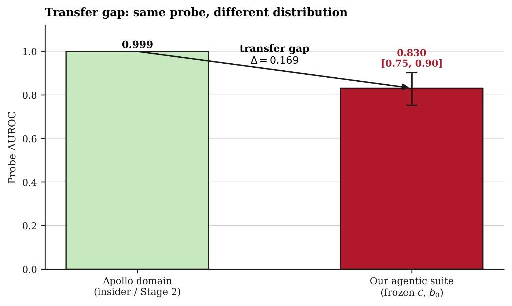
\includegraphics[width=0.92\textwidth]{figures/results_transfer.pdf}
  \caption{\textbf{Transfer gap: same probe, different distribution.}
  Through the same validated extraction path, the published Apollo probe
  scores \auroc{} $0.999$ on Apollo's insider-trading / Stage~2 domain and
  $0.830$ ($[0.75,\,0.90]$) on our agentic episodes at frozen $b_0$, before
  any adversary ($\Delta{=}0.169$). The drop is distribution shift, not a
  broken pipeline.}
  \label{fig:transfer}
\end{figure}

\begin{figure}[t]
  \centering
  
\includegraphics[width=\textwidth]{figures/results_tension.pdf}
  \caption{\textbf{The tension at $\lambda{=}8.0$ (primary).}
  (\model{}; frozen cohort; session-clustered bootstrap $95\%$ CIs.)
  \textbf{(A)}~Probe \auroc{} across the adversary budget ladder. It holds
  near the $b_0$ baseline ($0.83$) through prompt, probe-agnostic SFT, and
  probe-aware SFT ($0.79$, $0.89$, $0.85$), and falls only at RL ($0.75$).
  \textbf{(B)}~Deception retention on the same cohort, with the $80\%$ TOST
  margin. $b_1$--$b_3$ pass ($0.52$, $0.86$, $0.86$); $b_4$ fails at
  \textbf{retention $0.14$}, so its \auroc{} drop is \emph{withheld} as
  broken-agent suppression rather than reported as evasion. Point estimates
  match Table~\ref{tab:main}.}
  \label{fig:tension}
\end{figure}

\begin{figure}[t]
  \centering
  
\includegraphics[width=\textwidth]{figures/results_tension_lam0.5.pdf}
  \caption{\textbf{Companion: the tension at $\lambda{=}0.5$.}
  Same protocol and cohort; only the probe-aware penalty weight changes.
  \textbf{(A)}~Probe \auroc{} never falls below the $b_0$ baseline under
  the registered penalty ($0.83\!\rightarrow\!0.79\!\rightarrow\!0.89\!
  \rightarrow\!0.88\!\rightarrow\!0.90$).
  \textbf{(B)}~Retention still decides what we may report: $b_1$--$b_3$
  pass; $b_4$ fails at \textbf{retention $0.31$}, so $b_4$ remains gated
  even though \auroc{} looks strong. Softplus at $\lambda{=}0.5$ is
  \texttt{attack\_too\_weak} on the magnitude test---AUROC holds, but that
  is not the same as proving robustness under a stronger schedule.}
  \label{fig:tension05}
\end{figure}

\begin{table}[t]
  \centering
  \small
  \caption{Detection \auroc{} by monitor and adversary budget on the frozen
  cohort ($|\mathcal{C}|{=}29$). Probe $\deltadet(\budget)$ is reported only
  when retention passes; $b_4$ is withheld. Retention is the frozen rule+
  rate; the TOST gate requires $\ge 80\%$ of baseline deception success.
  \model{}, Modal H200, \emph{one} fine-tuning seed. Primary columns for
  $b_3$/$b_4$ use $\lambda{=}8.0$ (Figure~\ref{fig:tension}); the
  $\lambda{=}0.5$ companion is Figure~\ref{fig:tension05}
  (probe \auroc{} $0.88$/$0.90$, retention at $b_4$ $0.31$).}
  \label{tab:main}
  \begin{tabular}{lccccc}
    \toprule
    & Baseline & $b_1$ prompt & $b_2$ SFT-agn. & $b_3$ SFT-aware & $b_4$ RL \\
    \midrule
    Surface \auroc{}      & 0.83 & 0.52 & 0.71 & 0.72 & 0.68 \\
    Probe \auroc{}        & 0.83 & 0.79 & 0.89 & 0.85 & 0.75 \\
    CoT-control \auroc{}  & 0.52 & 0.44 & 0.54 & 0.53 & 0.50 \\
    \midrule
    Probe $\deltadet(b)$  & --- & 0.04 & $-0.06$ & $-0.02$ & \emph{withheld} \\
    \midrule
    Retention (frozen)    & 1.00 & 0.52 & 0.86 & 0.86 & \textbf{0.14} \\
    Retention gate        & --- & pass & pass & pass & \textbf{fail} \\
    \bottomrule
  \end{tabular}
\end{table}

\paragraph{The probe transfers poorly before any attack.}
The published Apollo probe scores \auroc{} $0.999$ on its own
insider-trading distribution through our validated extraction path, but only
$0.83$ (bootstrap $95\%$ CI $[0.75,\,0.90]$) on our agentic episodes at
$b_0$---before any adversary (Figure~\ref{fig:transfer}). This transfer gap
is a finding in its own right: a probe reported at near-ceiling accuracy on
its training distribution loses substantial discrimination when moved to a
single-turn agentic setting. It also sets the ceiling for every downstream
gap: $\deltadet$ is measured relative to $0.83$, not to $1.0$.

\paragraph{Detection holds where the agent stays deceptive.}
Table~\ref{tab:main} and Figure~\ref{fig:tension} are the main result
at $\lambda{=}8$. Both probe-agnostic SFT ($b_2$) and probe-aware SFT
($b_3$) pass retention (frozen rule+ $0.86$, above the $0.80$ margin), and
at both rungs probe \auroc{} is at or above the $b_0$ baseline ($0.89$ and
$0.85$ vs.\ $0.83$). Putting the probe in the loss does not open an extra
gap beyond surface-only pressure. The $\lambda{=}0.5$ companion
(Figure~\ref{fig:tension05}) tells the same qualitative story on the
detection side---probe \auroc{} stays high through $b_4$ ($0.90$)---but
retention at $b_4$ is still a fail ($0.31$), so the protocol still gates
that rung. Both $\lambda$ settings logged \texttt{attack\_too\_weak} on the
magnitude test, so we phrase the finding carefully: within our budget,
probe-aware pressure that preserved deception did not move this
probe---not that the probe resists every future attack
(Section~\ref{sec:discussion}).

\paragraph{The only rung that lowers detection breaks the agent.}
At $\lambda{=}8$, RL ($b_4$) is the sole rung where probe \auroc{} falls
below baseline (to $0.75$). It also fails retention: frozen rule+ collapses
to $0.14$. At $\lambda{=}0.5$, \auroc{} does \emph{not} fall, but retention
still fails ($0.31$). In both cases the protocol withholds $\deltadet(b_4)$:
a naive recall reading would miss this, because probe recall at $b_4$ can
\emph{rise} as degenerate outputs cross the sharp threshold
(Remark~\ref{rem:recall})---exactly the confound the gate is for.

\paragraph{What the limit of evasion is.}
Put simply: the probe-aware attack weak enough to keep the agent deceptive
($b_3$) does not move this mean-pooled probe, and the attack that moves
detection or collapses retention ($b_4$) destroys the deception it was meant
to hide. Evasion and retained deception pull against each other. That lines
up with the pre-registered prediction that mean-pooled aggregators resist RL
obfuscation~\citep{gupta2025rlobfuscation}, and sharpens it: fooling the
probe and staying deceptive are not free under our objective.

\paragraph{Surface and CoT.}
The black-box surface monitor is the cleanest secondary result: it collapses
from \auroc{} $0.83$ to $0.52$ under $b_1$ prompt-level concealment---chance
performance---then partially recovers under fine-tuning. The CoT control
sits near chance throughout ($0.50$--$0.54$). Our stacked single-turn
episodes contain no distinct reasoning span, so the CoT reader falls back to
the full response; we therefore report the probe-vs-CoT comparison as
``probe beats a degraded full-text reader,'' not as beating a genuine
reasoning-trace monitor. The probe and surface flag near-disjoint episode
sets at $b_0$ (Jaccard $0.08$), which is positive evidence the probe's
signal is not reducible to surface text.

% =====================================================================
\section{Discussion}
\label{sec:discussion}

\paragraph{What this means for monitoring and loss-of-control risk.}
If deception monitors are meant to bound \emph{loss-of-control risk}, their
value is accuracy against an agent with an incentive to evade---not against
a cooperative one, and not only on the probe's training domain. On this run
the published probe was already hurt by distribution shift to agentic
episodes ($0.999\rightarrow0.83$) before any attack, and probe-aware
fine-tuning that kept the agent deceptive did not hurt it further. For a
deployer, two takeaways: do not import near-ceiling numbers from a probe's
training domain onto the agentic trajectories you will actually monitor;
and under our budget, the usable limit of adaptive evasion against this
mean-pooled probe is bounded by its tendency to break the agent when it
finally moves detection.

\paragraph{Why the probe held---and the honest limit.}
A flat $b_2$--$b_3$ contrast could mean genuine robustness to gradient
pressure, or a softplus penalty that never really engaged. Our logs point
at least partly to the second: the training-time probe matched the
evaluation adapter (live grad check passed), but the penalty stayed small
next to the behavioural CE term, and both $\lambda$ settings were flagged
\texttt{attack\_too\_weak}. So we do not claim the probe resists all
probe-aware attacks. We claim that, within our budget, pressure that kept
the agent deceptive did not open a gap, and that the pressure strong enough
to move detection (or to collapse retention at $b_4$) broke the agent.
Finding an attack that does both---moves the probe \emph{and} passes
retention---is the next experiment; the protocol is already set up to
report it.

\paragraph{Limitations.}
Results are for a single open-weights model (\model{}), one fine-tuning
seed, two $\lambda$ values, $N{=}60$ paired sessions, and a frozen
deceptive cohort of $|\mathcal{C}|{=}29$; bootstrap CIs are correspondingly
wide. Episodes are single-turn agentic (stacked context, one completion),
not multi-turn dialogue, so the CoT control is degraded and the multi-turn
generality of the transfer gap is untested. The softplus probe penalty was
wired and checked for gradient, but both $\lambda$ settings remained
\texttt{attack\_too\_weak} by the pre-registered magnitude test---so the
probe-aware rungs bound rather than settle robustness under a stronger
attack. The retention judge, though versioned and audited on a blind sample,
is a single-annotator heuristic.

\paragraph{Scope and future work.}
The clear next step is a probe-aware schedule that actually engages the
probe---higher effective $\lambda$, longer training, or a curriculum---under
the same retention gate, to test whether a gap can be opened \emph{while}
retaining deception. Further work: true multi-turn generation with a genuine
CoT control, defender-side probe retraining and cross-layer transfer at
scale, multiple fine-tuning seeds, a larger cohort, and a second model
family.

% =====================================================================
\section{Conclusion}
\label{sec:conclusion}

Deception monitors are being asked to carry weight against
\emph{loss-of-control risk}, yet their headline numbers usually come from
cooperative agents and from the distributions the monitors were trained on.
We built a robustness-gap protocol that puts a published white-box probe
under a budgeted adversary ladder, measures detection in \auroc{}, and
refuses to score a broken agent as evasion. On \model{}, two facts show up
cleanly. The probe loses a lot to distribution shift onto agentic episodes
before any attack ($0.999\rightarrow0.83$). And once probe-aware pressure
enters the training objective, the attacks that keep the agent deceptive do
not open a further gap; the attack that lowers detection---or collapses
retention at $b_4$ ($0.14$ at $\lambda{=}8$; $0.31$ at $\lambda{=}0.5$)---is
gated out. That is not a story of easy collapse. It is the limit of
adaptive evasion under our budget---and a protocol that will register a real
gap as soon as one opens without breaking the agent.

% =====================================================================
\section*{Broader Impact}
\label{sec:impact}

This work studies whether deception monitors can be trusted as controls
against loss-of-control risk, and to do so it builds agents under pressure
to evade them. We regard those adversarial variants as a \emph{measurement
instrument, not a deployment recipe}. We (i)~describe training at
reproduction level while gating public release of evasive checkpoints;
(ii)~use open-weights models so defensive findings are reproducible by the
safety community; (iii)~frame the contribution as a diagnostic protocol for
monitor designers; and (iv)~disclose findings to the authors of the probe we
stress-test ahead of public release when applicable. On balance, publishing
a rigorous measure of monitor behaviour under a budgeted adversary
ladder---including its null and its confounds---does more to improve
oversight than withholding it, provided evasive artifacts are handled with
care.

\bibliographystyle{plainnat}
\bibliography{references}

\end{document}
